\documentclass[mat1]{fmfdelo}
% \documentclass[fin1]{fmfdelo}
% \documentclass[isrm1]{fmfdelo}
% \documentclass[mat2]{fmfdelo}
% \documentclass[fin2]{fmfdelo}
% \documentclass[isrm2]{fmfdelo}

% naslednje ukaze ustrezno napolnite
\avtor{Tom Gornik}

\naslov{Izrek o invarianci odprtih množic}
\title{Domain invariance theorem}

% navedite ime mentorja s polnim nazivom: doc.~dr.~Ime Priimek,
% izr.~prof.~dr.~Ime Priimek, prof.~dr.~Ime Priimek
% uporabite le tisti ukaz/ukaze, ki je/so za vas ustrezni
\mentor{ izr.~prof.~dr.~Jaka Smrekar}
% \mentorica{}
% \somentor{}
% \somentorica{}
% \mentorja{}{}
% \mentorici{}{}

\letnica{2020} % leto diplome

%  V povzetku na kratko opišite vsebinske rezultate dela. Sem ne sodi razlaga organizacije dela --
%  v katerem poglavju/razdelku je kaj, pač pa le opis vsebine.
\povzetek{}

%  Prevod slovenskega povzetka v angleščino.
\abstract{}

% navedite vsaj eno klasifikacijsko oznako --
% dostopne so na www.ams.org/mathscinet/msc/msc2010.html
\klasifikacija{}
\kljucnebesede{} % navedite nekaj ključnih pojmov, ki nastopajo v delu
\keywords{} % angleški prevod ključnih besed

\zapisiMetaPodatke  % poskrbi za metapodatke in veljaven PDF/A-1b standard

% aktivirajte pakete, ki jih potrebujete
\usepackage{tikz, verbatim, subcaption}
\usetikzlibrary{arrows.meta, calc}

% za številske množice uporabite naslednje simbole
\newcommand{\R}{\mathbb R}
\newcommand{\N}{\mathbb N}
\newcommand{\Z}{\mathbb Z}
\newcommand{\C}{\mathbb C}
\newcommand{\Q}{\mathbb Q}


% matematične operatorje deklarirajte kot take, da jih bo Latex pravilno stavil
% \DeclareMathOperator{\conv}{conv}

% vstavite svoje definicije ...
%  \newcommand{}{}
\newcommand{\I}{\mathbb I}
\newcommand{\0}{\underline{0}}
\newcommand{\Int}{\text{Int}}


\begin{document}
%####################     1. POGLAVJE: UVOD     ####################
\section{Uvod}
Koncept dimenzije prostora se zdi zelo naraven in intuitiven. V svojih zapisih je o dimenzijah govoril že Aristotel. A ko beremo njegova dela, hitro vidimo, da je bila njegova predstava o dimenzijah drugačna od današnje. Aristotel namreč pravi ,,Premica ima magnitudo v eni smeri, ravnina v dveh smereh, geometrijska telesa pa v treh smereh in poleg teh treh magnitud ni nobene več, kajti te tri so vse''. Matematiki so dolgo živeli v prepričanju, do so lahko matematični objekti največ tridimenzionalni. Kasneje so se začele pojavljati potrebe po štiridimenzionalnih objektih, saj so bile na primer v mehaniki enačbe veliko lažje, če je eno dimenzijo predstavljal čas. Tako smo počasi prišli do razmišljanja, da imamo večdimenzionalne in celo neskončno dimenzionalne prostore. Problem se pojavi, ko želimo primerjati prostore različnih dimenzij. Intuicija nam pravi, da prostora različnih dimenzij ne moreta biti enaka. V topologiji rečemo, da ne moreta biti homeomorfna. Homeomorfizem je bijektivna zvezna preslikava $f$, katere inverz $f^{-1}$ je tudi zvezen. Če lahko prostor $X$ z neko homeomorfno prelikavo preslikamo v prostor $Y$, pravimo, da sta prostora $X$ in $Y$ homeomorfna. Matematiki so že od nekdaj verjeli, da je dimenzija invarianta, kar pomeni, da imata homeomorfna prostora enako dimenzijo. To trditev je bilo zelo težko dokazati ne samo zato, ker je dokaz zapleten, ampak tudi zato, ker ni bilo dobre definicije dimenzije prostora? Govorimo o dimenzijah, o njih imamo neke predstave, a kaj sploh je dimenzija prostora? Velikokrat na dimenzijo gledamo kot na najmanjše število parametrov, ki so potrebni za opis nekega prostora. Ob tej definiciji smo lahko pomirjeni samo dokler ne spoznamo  Ko hočemo to dejstvo dokazati, spoznamo, da je to za višje dimenzije precej težje, kot se zdi na prvi pogled. Še večja zmeda nastane, ko spoznamo Peanove krivulje, ki enodimenzionalen prostor zvezno preslikajo v dvodimenzionalnega.

V tem delu bomo predstavili dokaz tega izreka. Brouwer je uporabil zahtevne topološke rezultate, mi pa bomo podali bolj elementaren dokaz, ki ga lahko razume študent dodiplomskega študija ali pa ljubiteljski matematik. V poglavjih 2-4 bomo spoznali nekaj matematičnih rezultatov, ki jih bomo potrebovali pri dokazu, v 5. poglavju pa bomo podali dokaz. Neučakan bralec lahko prebere najprej tudi to poglavje in se kasneje vrne nazaj ter naknadno zapolni vse vrzeli v dokazu.

%####################     2. POGLAVJE: SIMPLEKSI     ####################
\section{Simpleksi}
V tem razdelku bomo spoznali simplekse in z njimi povezano Spernerjevo lemo. Simpleks si lahko predstavljamo, kot posplošitev pojma trikotnik, ki je dvodimenzionalen objekt, na ostale dimenzije. Tako v $0$-dimenzionalnem prostoru simpleks označuje točko, enodimenzijonalen simpleks nam predstavlja daljico, v dveh dimenzijah dobimo že znani trikotnik, v treh dimenzijah pa simpleks imenujemo tudi tetraeder itn. Na sliki \ref{fig:simplex} so prikazani simpleksi dimenzij $0$, $1$, $2$, in $3$.
\begin{figure}[h!]  %####################   Simpleksi v različnih dimenzijah    ####################
	\centering
	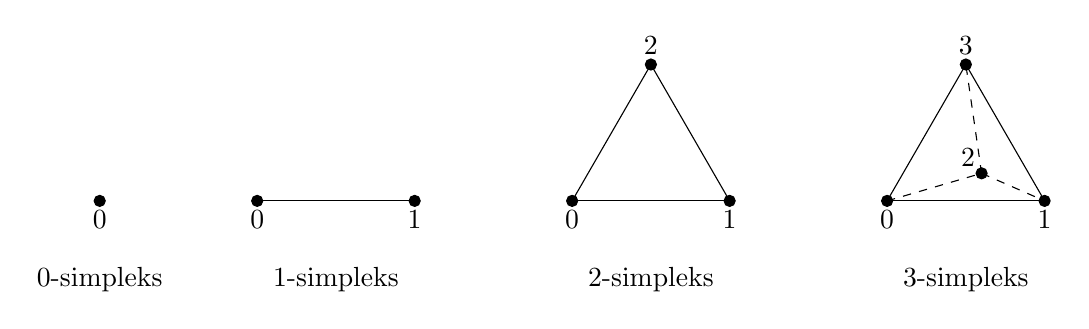
\begin{tikzpicture}
% ####################   0 - simplex    ####################
		\filldraw[black] (0, 0) circle (2pt) node[black, below]{$0$};
		\draw (0, -1) node {$0$-simpleks};
% ####################   1 - simplex    ####################
		\filldraw[black] (2, 0) circle (2pt) node[black, below]{$0$};		
		\filldraw[black] (4, 0) circle (2pt) node[black, below]{$1$};
		\draw (2, 0) -- (4, 0);
		\draw (3, -1) node {$1$-simpleks};
% ####################   2 - simplex    ####################
		\filldraw[black] (6, 0) circle (2pt) node[black, below]{$0$};		
		\filldraw[black] (8, 0) circle (2pt) node[black, below]{$1$};
		\filldraw[black] (7, 1.732) circle (2pt) node[black, above]{$2$};
		\draw (6, 0) -- (8, 0);
		\draw (6, 0) -- (7, 1.732);
		\draw (7, 1.732) -- (8, 0);
		\draw (7, -1) node {$2$-simpleks};
% ####################   3 - simplex    ####################
		\filldraw[black] (10, 0) circle (2pt) node[black, below]{$0$};		
		\filldraw[black] (12, 0) circle (2pt) node[black, below]{$1$};
		\filldraw[black] (11.2, 0.35) circle (2pt) node[black, above left = -0.4mm]{$2$};
		\filldraw[black] (11, 1.732) circle (2pt) node[black, above]{$3$};				
		\draw (10, 0) -- (12, 0);
		\draw (10, 0) -- (11, 1.732);
		\draw (11, 1.732) -- (12, 0);
		\draw[dashed] (10, 0) -- (11.2, 0.35);
		\draw[dashed] (11.2, 0.35) -- (11, 1.732);
		\draw[dashed] (11.2, 0.35) -- (12, 0);
		\draw (11, -1) node {$3$-simpleks};
	\end{tikzpicture}
	\caption{Simpleksi v dimenzijah $0$, $1$, $2$ in $3$}\label{fig:simplex}
\end{figure}
 Preden podamo natančno definicijo simpleksa, moramo spoznati afino neodvisne množice. Pri tem se bomo držali pravila, da bomo krajevni vektor od izhodišča do neke točke označili z enako oznako kot točko samo, le da bomo nad oznako narisali puščico. Torej krajevni vektor neke točke $x \in \R^n$ bomo označili z $\vec{x}$.
\begin{definicija}
Množica točk $x_0, x_1, \dots , x_{n-1} \in \R^n$ je \emph{afino neodvisna}, če je množica vektorjev $\vec{x}_1 - \vec{x}_0, \vec{x}_2 - \vec{x}_0, \dots , \vec{x}_{n-1} - \vec{x}_0$ linearno neodvisna.
\end{definicija}

Opazimo lahko, da ima v tej definiciji prva točka iz množice posebno vlogo. Ker ne govorimo o urejenih množicah in vrstni red elementov ni pomemben, se moramo prepričati, da nam definicija res karakterizira afino neodvisne množice in ni odvisna od izbire prve točke. Denimo, da je množica vektorjev $\vec{x}_1 - \vec{x}_0, \vec{x}_2 - \vec{x}_0, \dots , \vec{x}_{n-1} - \vec{x}_0$ linearno neodvisna. Potem je enakost $\sum\limits_{i=1}^{n-1} \alpha_i (\vec{x}_i - \vec{x}_0) = 0$ izpolnjena natanko tedaj, ko so vsi koeficienti enaki $0$, torej velja $\alpha_i = 0$ za vsak $i \in \{ 1, 2, \dots, n - 1 \}$ . Recimo, da smo za prvi element izbrali neko drugo točko na primer $x_k$. Radi bi videli, da je potem tudi enakost $\sum\limits_{\substack{i=0 \\ i\neq k}}^{n-1} \beta_i (\vec{x}_i - \vec{x}_k) = 0$ izpolnjena samo v primeru, ko so vsi koeficienti enaki $0$. V to se prepričamo tako, da uporabimo znan matematični trik ter odštejemo in prištejemo isto vrednost.
Računamo:
\begin{align*} 
\sum\limits_{\substack{i=0 \\ i \neq k}}^{n-1} \beta_i (\vec{x}_i - \vec{x}_k) &=  \sum\limits_{\substack{i=0 \\ i \neq k}}^{n-1} \beta_i (\vec{x}_i - \vec{x}_0 + \vec{x}_0 - \vec{x}_k) = \\
&=\sum\limits_{\substack{i=0 \\ i\neq k}}^{n-1} \beta_i (\vec{x}_i - \vec{x}_0) + \sum\limits_{\substack{i=0 \\ i\neq k}}^{n-1} \beta_i (\vec{x}_0 - \vec{x}_k) \\
&= \sum\limits_{i=1}^{n-1} \gamma_i (\vec{x}_i - \vec{x}_0),
\end{align*}
kjer koeficiente $\gamma_i$ določimo na naslednji način:
\[  \gamma_i =  \left\{
\begin{array}{cl}\vspace{3pt}
	-\sum\limits_{\substack{i=0 \\ i\neq k}}^{n-1} \beta_i & i = k,\\
	\beta_i & i \neq k. \\
\end{array} 
\right. \]
Ker je množica vektorjev $\vec{x}_1 - \vec{x}_0, \vec{x}_2 - \vec{x}_0, \dots , \vec{x}_{n-1} - \vec{x}_0$ linearno neodvisna, morajo biti vsi koeficienti $\gamma_i = 0$ za vsak $i \in \{1, 2, \dots, n-1\}$. Torej so tudi vsi koeficienti $\beta_i = 0$, za vsak $i \in \{0, 1, \dots, k-1, k+1, \dots, n-1\}$. Pokazali smo linearno neodvisnost množice $\vec{x}_0 - \vec{x}_k, \vec{x}_1 - \vec{x}_k, \dots , \vec{x}_{k-1} - \vec{x}_k, \vec{x}_{k+1} - \vec{x}_k, \dots, \vec{x}_{n-1} - \vec{x}_k$, zato je zgornja definicija dobra. 
Poglejmo si zdaj še definicijo simpleksa.
\begin{definicija}
Naj bo $V = \{x_0, x_1, \dots , x_{n-1} \} \subset \R^n$ afino neodvisna množica točk v Evklidskem prostoru $\R^n$. Množici 
$$S = \left\{\sum\limits_{i=0}^{n-1} \lambda_i \vec{x}_i; \text{ kjer je } \sum\limits_{i=0}^{n-1} \lambda_i = 1 \text{ in } \lambda_i \in [0, \infty) \text{ za vsak } i \in \{0, 1, \dots, n-1 \}\right\}$$
pravimo \emph{$n$-dimenzionalni simpleks} ali \emph{$n$-simpleks}.
\end{definicija}
Točkam $x_i$, ki določajo simpleks $S$, pravimo \emph{oglišča} simpleksa $S$. Krajevni vektor vsake točke $x \in S$ lahko torej zapišemo vsoto $\vec{x} = \sum\limits_{i=0}^{n-1} \lambda_i \vec{x}_i$, ki zadošča pogoju $\sum\limits_{i=0}^{n-1} \lambda_i = 1$, kjer so vsi $\lambda_i$ pozitivna realna števila. Vsoto, ki zadošča zahtevanim pogojem imenujemo \emph{afina kombinacija} točk $x_0, x_1, \dots , x_{n-1}$. Števila $\lambda_i$ pa so \emph{baricentrične koordinate} točke $x$.

1

1


Pri dokazovanju različnih rezultatov s pomočjo simpleksov si večkrat pomagamo z delitvijo simpleksa na manjše simplekse. Da pa imamo čimveč nadzora pri dokazovanju, definiramo posebno delitev simpleksa, ki jo imenujemo triangulacija.

\begin{definicija}
\emph{Triangulacija} $T$ $n$-simpleksa $S$ je vsaka množica $n$-simpleksov, za katero veljata naslednji lastnosti:
\begin{enumerate}
\item Neprazen presek $L$ dveh simpleksov je lice obeh simpleksov in velja $L \in T$.
\item Unija vseh simpleksov iz $T$ enaka $S$
\end{enumerate}
\end{definicija}
% ####################   Primer triangulacije    ####################
\begin{figure}[h]  
\centering 
	\begin{subfigure}[b]{0.4\linewidth}
		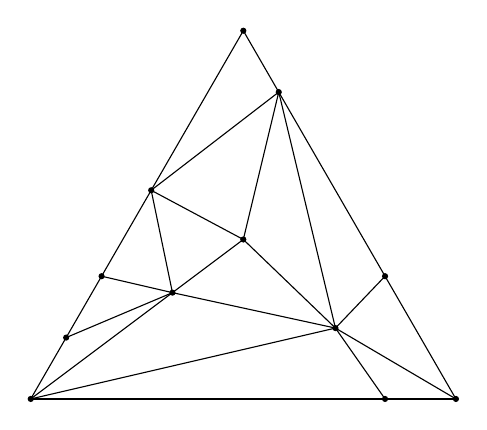
\begin{tikzpicture}[scale=0.9]
			\filldraw[black] (0, 0) circle (1pt);
			\filldraw[black] (2, 1.5) circle (1pt);
			\filldraw[black] (1.7, {1.7*sqrt(3)}) circle (1pt);
			\filldraw[black] (3.5, {2.5*sqrt(3)}) circle (1pt);
			\filldraw[black] (3, 2.25) circle (1pt);
			\filldraw[black] (5, 0) circle (1pt);
			\filldraw[black] (6, 0) circle (1pt);
			\filldraw[black] (3, {3*sqrt(3)}) circle (1pt);
			\filldraw[black] (5, {sqrt(3)}) circle (1pt);
			\filldraw[black] (0.5, {0.5*sqrt(3)}) circle (1pt);
			\filldraw[black] (4.3, 1) circle (1pt);
			\filldraw[black] (1, {1*sqrt(3)}) circle (1pt);
			\draw (0, 0) -- (6, 0);
			\draw (0, 0) -- (3, 2.25);
			\draw (6, 0) -- (3, {3*sqrt(3)});
			\draw (3, {3*sqrt(3)}) -- (0, 0);
			\draw (4.3, 1) -- (6, 0);
			\draw (0, 0) -- (4.3, 1);
			\draw (4.3, 1) -- (5, {sqrt(3)});
			\draw (4.3, 1) -- (5, 0);
			\draw (4.3, 1) -- (3.5, {2.5*sqrt(3)});
			\draw (4.3, 1) -- (2, 1.5);
			\draw (4.3, 1) -- (3, 2.25);
			\draw (1.7, {1.7*sqrt(3)}) -- (3, 2.25);
			\draw (2, 1.5) -- (0.5, {0.5*sqrt(3)});
			\draw (2, 1.5) -- (1.7, {1.7*sqrt(3)});
			\draw (3.5, {2.5*sqrt(3)}) -- (3, 2.25);
			\draw (3.5, {2.5*sqrt(3)}) -- (1.7, {1.7*sqrt(3)});
			\draw (2, 1.5) -- (1, {1*sqrt(3)});
		\end{tikzpicture}%
		\caption{Triangulacija} \label{fig:triang}
	\end{subfigure}
	\hspace{1cm}
	\begin{subfigure}[b]{0.4\linewidth}
		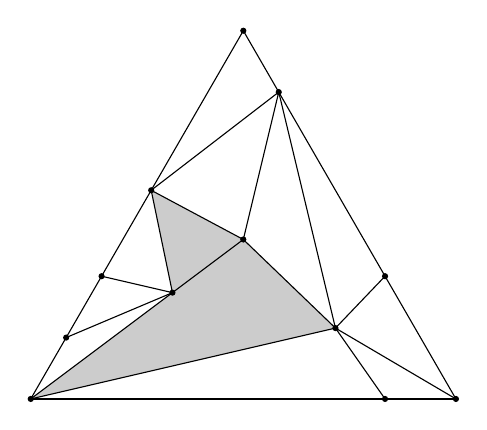
\begin{tikzpicture}[scale=0.9]
% ####################   Primer delitve, ki ni triangulacija    ####################
			\fill[fill=gray!40] (0, 0) -- (4.3, 1) -- (3, 2.25);
			\fill[fill=gray!40] (1.7, {1.7*sqrt(3)}) -- (2, 1.5) -- (3, 2.25);
			\filldraw[black] (0, 0) circle (1pt);
			\filldraw[black] (2, 1.5) circle (1pt);
			\filldraw[black] (1.7, {1.7*sqrt(3)}) circle (1pt);
			\filldraw[black] (3.5, {2.5*sqrt(3)}) circle (1pt);
			\filldraw[black] (3, 2.25) circle (1pt);
			\filldraw[black] (5, 0) circle (1pt);
			\filldraw[black] (6, 0) circle (1pt);
			\filldraw[black] (3, {3*sqrt(3)}) circle (1pt);
			\filldraw[black] (5, {sqrt(3)}) circle (1pt);
			\filldraw[black] (0.5, {0.5*sqrt(3)}) circle (1pt);
			\filldraw[black] (4.3, 1) circle (1pt);
			\filldraw[black] (1, {1*sqrt(3)}) circle (1pt);
			\draw (0, 0) -- (6, 0);
			\draw (0, 0) -- (3, 2.25);
			\draw (6, 0) -- (3, {3*sqrt(3)});
			\draw (3, {3*sqrt(3)}) -- (0, 0);
			\draw (4.3, 1) -- (6, 0);
			\draw (0, 0) -- (4.3, 1);
			\draw (4.3, 1) -- (5, {sqrt(3)});
			\draw (4.3, 1) -- (5, 0);
			\draw (4.3, 1) -- (3.5, {2.5*sqrt(3)});
			\draw (4.3, 1) -- (3, 2.25);
			\draw (1.7, {1.7*sqrt(3)}) -- (3, 2.25);
			\draw (2, 1.5) -- (0.5, {0.5*sqrt(3)});
			\draw (2, 1.5) -- (1.7, {1.7*sqrt(3)});
			\draw (3.5, {2.5*sqrt(3)}) -- (3, 2.25);
			\draw (3.5, {2.5*sqrt(3)}) -- (1.7, {1.7*sqrt(3)});
			\draw (2, 1.5) -- (1, {1*sqrt(3)});
		\end{tikzpicture}
		\caption{Ni triangulacija} \label{fig:nitriang}  
	\end{subfigure}
\caption{Primer in protiprimer triangulacije simpleksa.}
\end{figure} 

Včasih imamo zaradi lažje predstave raje bolj simetrične triangulacije.

\begin{definicija}
Kadar je simpleks $S$ razdeljen s skladnimi simpleksi, govorimo o baricentrični triangulaciji. Za vsako naravno število $k \in \N$ lahko definiramo triangulacijo, ki ima za $0$-simplekse množico 
$$V_k = \left\{\sum\limits_{i=0}^{n-1} \frac{\lambda_i}{k} x_i, \text{ kjer je } \sum\limits_{i=0}^{n-1} \lambda_i = k \text{ in } \lambda_i \in [0, \infty) \text{ za vsak } i = 0, 1, \dots, n-1 \right\}.$$
Taki triangulaciji pravimo \emph{$k$-baricentrična triangulacija} simpleksa.
\end{definicija}

\begin{definicija}
Naj bo podan $n$-simpleks $S \in \R^n$ s triangulacijo $T$. Označimo množico $0$-simpleksov iz $T$ z $V$.
Barvanje triangulacije $T$ je preslikava $b : V \to \left \{1, 2, \dots, n+1 \right \} $.  
\end{definicija}

\begin{definicija}
Če j
\end{definicija}


\begin{lema}[Spernerjeva lema]\label{izr:sperner}
V vsaka triangulacija $k$-simpleksa s spernerjevim barvanjem vsebuje liho število popolno pobarvanih $k$-simpleksov.
\end{lema}
\begin{proof}
Naj bo $S$ $k$-simpleks in naj bo $T$ njegova triangulacija. Lemo bomo dokazovali z indukcijo na dimenzijo simpleksa $k$. 
\begin{itemize}
\item
\underline{Baza indukcije ($k = 0$).}
Če je $k=0$, lema očitno drži, saj je $0$-simpleks točka. Pri spernerjevem barvanju točke, pa imamo samo eno možnost in tako dobimo en popolno pobarvan $0$-simpleks.
\item
\underline{Indukcijska predpostavka ($k - 1$).}
Predpostavimo, da lema drži v dimenziji $(k - 1)$. Torej v vsaki triangulaciji $(k - 1)$-simpleksa s spernerjevim barvanjem najdemo liho število $(k - 1)$-simpleksov, ki so popolno pobarvani. 
\item
\underline{Indukcijski korak ($(k - 1) \Longrightarrow k$).}
Poskusimo dakazati pravilnost izjave tudi v dimenziji $k$. Vzemimo poljubno triangulacijo $T$ $k$-simpleksa $S$. Naj bodo vozlišča triangulacije $T$ pobarvana s spernerjevim barvanjem. Označimo število vseh popolno pobarvanih $i$-simpleksov iz $T$ z $S_p^i$, število tistih popolno pobarvanih $i$-simpleksov, ki se nahajajo na robu simpleksa $S$ pa z $R_p^i$. Vsak popolno pobarvan $k$-simpleks vsebuje natanko en popolno pobarvan $(k-1)$-simpleks, medtem ko ostali simpleksi lahko vsebujejo dva ali pa nobenega. Če $k$-simpleks vsebuje vozlišča pobarvana z vsemi barvami $0, 1, \dots, k-2$, kjer se ena barva ponovi dvakrat, tak simpleks vsebuje dva popolno pobarvana simpleksa. Ostali simpleksi pa ne vsebujejo popolno pobarvanih $(k - 1)$-simpleksov. Iz zgornjega lahko sklepamo, da je $S_p^k \equiv S_p^{k-1} \pmod 2$. Pri štetju popolno pobarvanih $(k - 1)$-simpleksov smo vsakega iz notranjosti $S$ šteli dvakrat, tiste iz roba $S$ pa samo enkrat. Zato velja tudi $R_p^{k - 1} \equiv S_p^{k-1} \pmod 2$. Torej velja $R_p^{k - 1} \equiv S_p^{k-1} \pmod 2$. Popolno pobarvane $(k - 1)$-simplekse zaradi spernerjevega barvanja lahko najdemo zgolj na enem pravem licu $L$ simpleksa $S$. Po indukcijski predpostavki pa $L$ vsebuje liho mnogo popolno pobarvanih $(k - 1)$-simpleksov, kar pomeni, da je $R_p^{k - 1}$ liho število. Torej je tudi  $S_p^k$ lih.
\end{itemize}
\end{proof}

\begin{definicija}
Naj bo $a \in \R$ poljubno pozitivno realno število in naj bo $\I = \left [ -a, a \right ] $. Potem je $C := \I^n$ \emph{$n$-dimenzionalna kocka} v $\R^n$ oziroma \emph{$n$-kocka}.
\end{definicija}

\begin{definicija}
\emph{Triangulacija $T$ kocke} $C$ je taka množica simpleksov, za katero veljata naslednji lastnosti:
\begin{enumerate}
\item Unija vseh simpleksov iz $T$ enaka $C$.
\item Neprazen presek $L$ dveh simpleksov je lice obeh simpleksov in velja $L \in T$.
\end{enumerate}
\end{definicija}

\begin{definicija}
Spernerjevo barvanje kombinatorične kocke je preslikava 
\end{definicija}

\begin{lema}[Spernerjeva lema za kocke]\label{izr:kubsperner}
V vsakem spernerjevem barvanju triangulacije $k$-kocke je liho mnogo popolno pobarvanih $k$-simpleksov.
\end{lema}
\begin{proof}
Naj bo $C$ $k$-kocka in naj bo $T$ njegena triangulacija. Lemo bomo dokazovali z indukcijo na dimenzijo kocke $k$. 
\begin{itemize}
\item
\underline{Baza indukcije ($k = 0$).}
Če je $k=0$, lema očitno drži, saj je $0$-kocka točka. Pri spernerjevem barvanju točke, pa imamo samo eno možnost in tako dobimo eno popolno pobarvano $0$-kocko.
\item
\underline{Indukcijska predpostavka ($k - 1$).}
Predpostavimo, da lema drži v dimenziji $(k - 1)$. Torej v vsaki triangulaciji $(k - 1)$-kocke s spernerjevim barvanjem najdemo liho število $(k - 1)$-simpleksov, ki so popolno pobarvani. 
\item
\underline{Indukcijski korak ($(k - 1) \rightarrow k$).}
Poskusimo dakazati pravilnost izjave tudi v dimenziji $k$. Vzemimo poljubno triangulacijo $T$ $k$-simpleksa $S$. Naj bodo vozlišča triangulacije $T$ pobarvana s spernerjevim barvanjem. Označimo število vseh popolno pobarvanih $i$-simpleksov iz $T$ z $S_p^i$, število tistih popolno pobarvanih $i$-simpleksov, ki se nahajajo na robu simpleksa $S$ pa z $R_p^i$. Vsak popolno pobarvan $k$-simpleks vsebuje natanko en popolno pobarvan $(k-1)$-simpleks, medtem ko ostali simpleksi lahko vsebujejo dva ali pa nobenega. Če $k$-simpleks vsebuje vozlišča pobarvana z vsemi barvami $0, 1, \dots, k-2$, kjer se ena barva ponovi dvakrat, tak simpleks vsebuje dva popolno pobarvana simpleksa. Ostali simpleksi pa ne vsebujejo popolno pobarvanih $(k - 1)$-simpleksov. Iz zgornjega lahko sklepamo, da je $S_p^k \equiv S_p^{k-1} \pmod 2$. Pri štetju popolno pobarvanih $(k - 1)$-simpleksov smo vsakega iz notranjosti $S$ šteli dvakrat, tiste iz roba $S$ pa samo enkrat. Zato velja tudi $R_p^{k - 1} \equiv S_p^{k-1} \pmod 2$. Torej velja $R_p^{k - 1} \equiv S_p^{k-1} \pmod 2$. Popolno pobarvane $(k - 1)$-simplekse zaradi spernerjevega barvanja lahko najdemo zgolj na enem pravem licu $L$ simpleksa $S$. Po indukcijski predpostavki pa $L$ vsebuje liho mnogo popolno pobarvanih $(k - 1)$-simpleksov, kar pomeni, da je $R_p^{k - 1}$ liho število. Torej je tudi  $S_p^k$ lih.
\end{itemize}
\end{proof}



\newcommand*\rows{6}
\newcommand*\vel{1.8}
\begin{figure}[h!]    %####################   Spernerjevo barvanje    ####################
	\centering
	\begin{tikzpicture}
		\fill[fill=gray!25] ($\vel*(3.5, {0.5*sqrt(3)})$)--($\vel*(3, {sqrt(3)})$)--($\vel*(4, {sqrt(3)})$);
		\fill[fill=gray!25] ($\vel*(3, {sqrt(3)})$)--($\vel*(2.5, {1.5*sqrt(3)})$)--($\vel*(3.5, {1.5*sqrt(3)})$);
		\fill[fill=gray!25] ($\vel*(2.5, {2.5*sqrt(3)})$)--($\vel*(2, {2*sqrt(3)})$)--($\vel*(3, {2*sqrt(3)})$);
		\foreach \k in {0, 1, ...,\rows} {
			\draw ($\vel*\k*(0.5, {0.5 * sqrt(3)})$) -- ($\vel*(\rows, 0) + \vel*\k*(-0.5, {0.5 * sqrt(3)})$);
			\draw ($\vel*\k*(1, 0)$) -- ($\vel*(\rows/2,{\rows/2 * sqrt(3)}) + \vel*\k*(0.5, {-0.5 * sqrt(3)})$);
			\draw ($\vel*\k*(1, 0)$) -- ($(0,0) + \vel *\k*(0.5, {0.5 * sqrt(3)})$);
		}
		
		\filldraw[red] (0, 0) circle (5pt);
		\filldraw[red] (\vel, 0) circle (5pt);
		\filldraw[green] (2*\vel, 0) circle (5pt);
		\filldraw[green] (3*\vel, 0) circle (5pt);
		\filldraw[red] (4*\vel, 0) circle (5pt);
		\filldraw[green] (5*\vel, 0) circle (5pt);
		\filldraw[green] (6*\vel, 0) circle (5pt);
		
		\filldraw[blue] ($\vel*(0.5, {0.5*sqrt(3)})$) circle (5pt);
		\filldraw[red] ($\vel*(1.5, {0.5*sqrt(3)})$) circle (5pt);
		\filldraw[red] ($\vel*(2.5, {0.5*sqrt(3)})$) circle (5pt);
		\filldraw[green] ($\vel*(3.5, {0.5*sqrt(3)})$) circle (5pt);
		\filldraw[green] ($\vel*(4.5, {0.5*sqrt(3)})$) circle (5pt);
		\filldraw[blue] ($\vel*(5.5, {0.5*sqrt(3)})$) circle (5pt);
		
		\filldraw[red] ($\vel*(1, {sqrt(3)})$) circle (5pt);
		\filldraw[green] ($\vel*(2, {sqrt(3)})$) circle (5pt);
		\filldraw[red] ($\vel*(3, {sqrt(3)})$) circle (5pt);
		\filldraw[blue] ($\vel*(4, {sqrt(3)})$) circle (5pt);
		\filldraw[green] ($\vel*(5, {sqrt(3)})$) circle (5pt);

		\filldraw[red] ($\vel*(1.5, {1.5*sqrt(3)})$) circle (5pt);
		\filldraw[green] ($\vel*(2.5, {1.5*sqrt(3)})$) circle (5pt);
		\filldraw[blue] ($\vel*(3.5, {1.5*sqrt(3)})$) circle (5pt);
		\filldraw[blue] ($\vel*(4.5, {1.5*sqrt(3)})$) circle (5pt);
		
		\filldraw[red] ($\vel*(2, {2*sqrt(3)})$) circle (5pt);
		\filldraw[green] ($\vel*(3, {2*sqrt(3)})$) circle (5pt);
		\filldraw[green] ($\vel*(4, {2*sqrt(3)})$) circle (5pt);

		\filldraw[blue] ($\vel*(2.5, {2.5*sqrt(3)})$) circle (5pt);
		\filldraw[blue] ($\vel*(3.5, {2.5*sqrt(3)})$) circle (5pt);
		
		\filldraw[blue] ($\vel*(3, {3*sqrt(3)})$) circle (5pt);
		
		\foreach \k in {0, 1, ...,\rows} {
			\foreach \j in {0, ...,\k} {
				%\filldraw[white] ($\vel*(\rows-\k, 0) + \vel*\j*(0.5, {0.5*sqrt(3)})$) circle (5pt);
				\draw ($\vel*(\rows-\k, 0) + \vel*\j*(0.5, {0.5*sqrt(3)})$) circle (5pt);
			}
		}
		
		\draw ($\vel*(-0.8+\rows/4, {0.3+\rows/4 * sqrt(3)})$) node[rotate=60] {\text{Vozlišča pobarvana zgolj z rdečo in modro}};
		\draw ($\vel*(0.8+3*\rows/4, {0.3+\rows/4 * sqrt(3)})$) node[rotate=-60] {Vozlšča pobarvana zgolj z modro in zeleno};
		\draw (\vel*\rows/2, -1) node {Vozlišča pobarvana zgolj z rdečo in zeleno};
	\end{tikzpicture}
	\caption{Spernerjevo barvanje}
\end{figure}


\begin{figure}[h!]
	\centering
	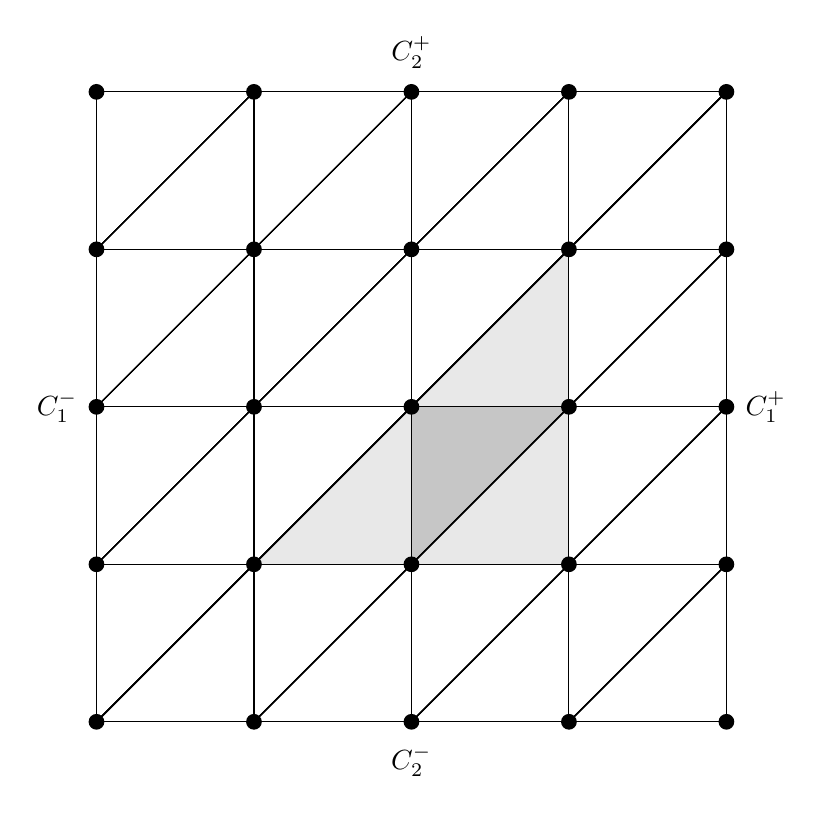
\begin{tikzpicture}
		\draw (0, 4.5) node {$C_2^+$};
		\draw (0, -4.5) node {$C_2^-$};
		\draw (4.5, 0) node {$C_1^+$};
		\draw (-4.5, 0) node {$C_1^-$};
		\fill[fill=gray!45] (0,0)--(0,-2)--(2,0);
		\fill[fill=gray!18] (0,0)--(2,0)--(2,2);
		\fill[fill=gray!18] (0,-2)--(2,-2)--(2,0);
		\fill[fill=gray!18] (0,0)--(0,-2)--(-2,-2);
		\foreach \x in {-4,-2,0,2,4}
		{   \foreach \y in {-4,-2,0,2,4}
		    {  \fill (\x,\y) circle (0.1cm);
		       \draw (-4, \y ) -- (4, \y );
		       \draw ( \x ,-4) -- ( \x ,4);
		       \draw ( -4 , \x) -- ( - \x ,4);
		       \draw ( \x , -4) -- ( 4 ,- \x );
		    }
		}
	\end{tikzpicture}
	\caption{Simpleksi}
\end{figure}

%####################     3. POGLAVJE: POINCARÉ--MIRANDOV IZREK     ####################
\section{Poincar\'{e}--Mirandov izrek}

\begin{izrek}[Poincar\'{e}-Mirandov izrek]\label{izr:PM}
Naj bo $a$ poljubno pozitivno realno število in naj bo $\mathbb{I}^n := [-a, a]^n$ hiperkocka v $\R^n$. Stranske ploskve ali lica hiperkocke $\mathbb{I}^n$ označimo z $\mathbb{I}_-^n = \{x\in \mathbb{I}^n | x_i = -a\}$ in $\mathbb{I}_+^n = \{x\in \mathbb{I}^n | x_i = a\}.$
 Naj bo $f : X \rightarrow \R^n$ taka zvezna preslikava iz kompaktnega prostora $X$ v evklidski prostor $\R^n$, da je za vsak $i \in \{1, \dots, n\}$ slika $f_i(\mathbb{I}_i^-) \subset (- \infty, 0] $ in  $f_i(\mathbb{I}_i^+) \subset [0, \infty) $. Potem obstaja $c \in \mathbb{I}^n$, da je za vsak $i \in \{1, \dots, n\}$ vrednost funkcije $f_i(c) = 0$.
\end{izrek}
Preden začnemo z dokazom Poincar\'{e}-Mirandovega izreka, si poglejmo, kako izgleda pogoj za funkcijo v dimenzijah $0$, $1$ in $2$.

\begin{figure}[h!]
	\centering
	\begin{tikzpicture}
% ####################   1 - D    ####################
		\filldraw[black] (0, 0) circle (2pt) node[black, left]{$I_1^-$};		
		\filldraw[black] (2, 0) circle (2pt) node[black, right]{$I_1^+$};
		\draw (0, 0) -- (2, 0);
% ####################   2 - D    ####################
		\draw (4, -1) -- (6, -1);
		\draw (4, -1) -- (4, 1);
		\draw (6, -1) -- (6, 1);
		\draw (4, 1) -- (6, 1);
		\draw (4, 0) node[black, left]{$I_1^-$};
		\draw (6, 0) node[black, right]{$I_1^+$};
		\draw (5, -1) node[black, below]{$I_2^-$};
		\draw (5, 1) node[black, above]{$I_2^+$};
% ####################   3 - D    ####################
		\draw (8, -1) -- (10, -1);
		\draw (10, -1) -- (10, 1);
		\draw (10, 1) -- (8, 1);
		\draw (8, 1) -- (8, -1);
		\draw[dashed] (8.7, -0.3) -- (10.7, -0.3);
		\draw (10.7, -0.3) -- (10.7, 1.7);
		\draw (10.7, 1.7) -- (8.7, 1.7);
		\draw[dashed] (8.7, 1.7) -- (8.7, -0.3);
		\draw[dashed] (8, -1) -- (8.7, -0.3);
		\draw (10.7, -0.3) -- (10, -1);
		\draw (10, 1) -- (10.7, 1.7);
		\draw (8, 1) -- (8.7, 1.7);
		\draw (8, 0.3) node[black, right]{$I_1^-$};
		\draw (10, 0.3) node[black, right]{{\large $I_1^+$\par}};
		\draw (9.15, -0.35) node[black, above]{{\large $I_2^-$\par}};
		\draw (9.65, 0.25) node[black, above]{$I_2^+$};
		\draw (9.4, -1.05) node[black, above]{$I_3^-$};
		\draw (9.4, 0.9) node[black, above]{{\large $I_3^+$\par}};
	\end{tikzpicture}
	\caption{Pogoji Poincar\'{e} - Mirandovega izreka}
\end{figure}

%####################     4. POGLAVJE: RAZŠIRITEV FUNKCIJE     ####################
\section{Razširitev funkcije}
\begin{definicija}
Diameter neprazne množice $A \subset \R^n$ označimo z $diam(A)$ je definiran kot $diam(A) = \sup \left \{ d(x, y) | x, y \in A \right \}$.
\end{definicija}

\begin{definicija}
Družini $\mathcal{A}$ podmnožic množice $X$, za katero velja $\bigcup_{A \in \mathcal{A}} = X$ pravimo pokritje množice $X$. Če družina $\mathcal{A}$ vsebuje zgolj odprte množice, jo imenujemo odprto pokritje množice $X$.
\end{definicija}

Predstavljajmo si zvezno funkcijo $f : X \to \R^n \setminus \{0\}$, ki slika iz kompaktne množice $K$ v evklidski prostor $\R^n \setminus \{ 0 \}$. Radi 

\begin{lema}[Razširitev funkcije]\label{razsiritev}
Naj bo $A$ kompaktna podmnožica evklidskega prostora $\R^n$ in naj bo \mbox{$f : A \to \R$}. Potem obstaja zvezna preslikava $F : \R^n \to \R$, da je za vsak $x \in A$, $f(x) = F(x)$.
\end{lema}

\begin{dokaz}
Včasih je pri dokazu obstoja neke stvari najlažje, če to stvar poiščemo in jo vsem pokažemo. Tako bomo tudi mi napisali predpis funkcije $F$, ki zvezno razširi funkcijo $f$. Seveda bi se lahko pri dokazu oprli na Tietzejev razširitveni izrek, a je to delo zasnovano tako, da se izogne abstraktnejšim topološkim delom. Denimo torej, da imamo kompaktno množico $K$ in zvezno funkcijo \mbox{$f : A \to \R$}.
Razširitveno funkcijo \mbox{$F : \R^n \to \R$} lahko definiramo s predpisom:
\[  F(x) = \left\{
\begin{array}{ll}
	\inf \left \{ f(a) + \frac{d(x, a)}{d(x, A)} - 1; a \in A \right \} &, x \in A^c \\
	f(x) &, x \in K. \\
\end{array} 
\right. \]
Enostavno se je prepričati, da je za vsak $x \in A$, $f(x) = F(x)$. Ugotoviti moramo le še, ali je funkcija $F$ res zvezna na $R^n$.
Dokazovali bomo v dveh delih. Najprej bomo dokazali zveznost funkcije $F$ na $A^c$, potem pa še na $A$.
Izberimo neko poljubno majhno pozitivno realno število $\varepsilon > 0$ in $x_0 \in A^c$. Potem obstaja tako pozitivno realno število $r>0$, da je odprta krogla s polmerom $r$ vsebovana v $A^c$, torej $B(x_0, r) \subset A^c$. Na $B(x_0, r)$ ja funkcija $D_a(x) := \frac{d(x, a)}{d(x, A)}$ zvezna za vsak parameter $a$, saj sta funkciji $d(x, a)$ in $d(x, A)$ zvezni in različni od $0$. Torej obstaja realno število $\delta \in (0, r)$, da je $|D_a(x_0) - D_a(x)| < \varepsilon$ za vsak $x \in B(x_0, \delta)$.
Denimo, da je infimum $f(x_0)$ dosežen pri $a_0$, torej je $F(x_0) = f(a_0) + D_{a_0}(x_0) - 1$. Za vrednosti $F(x)$ lahko naredimo naslednje ocene:
\begin{equation*} \label{eq1}
\begin{split}
F(x) & = F(x) - F(x_0) + F(x_0) = \\
& = \inf \left \{ f(a) + D_a(x) - 1; a \in A \right \} - F(x_0) + F(x_0) \leq \\
& \leq (f(a_0) + D_{a_0}(x) - 1) -  (f(a_0) + D_{a_0}(x_0) - 1) + F(x_0) = \\
& = (D_{a_0}(x) -  D_{a_0}(x_0)) + F(x_0) \leq \\
& \leq \varepsilon + F(x_0), \\
& \implies F(x_0) - F(x) \geq -\varepsilon.
\end{split}
\end{equation*}

Podobno ocenimo:
\begin{equation*} \label{eq1}
\begin{split}
F(x_0) & = F(x_0) - F(x) + F(x) = \\
& = F(x_0) - \inf \left \{ f(a) + D_a(x) - 1; a \in A \right \} + F(x) \leq \\
& \leq (f(a_0) + D_{a_0}(x_0) - 1) -  (f(a_0) + D_{a_0}(x) - 1) + F(x) = \\
& = (D_{a_0}(x_0) -  D_{a_0}(x)) + F(x) \leq \\
& \leq \varepsilon + F(x), \\
& \implies F(x_0) - F(x) \leq \varepsilon.
\end{split}
\end{equation*}
Iz zgornjih ocen ugotovimo, da je $|F(x_0) - F(x)| \leq \varepsilon$, kar zagotavlja zveznost funkcije $F$ na $A^c$.

Da bi preverili zveznost $F$ tudi na množici $A$ izberemo $x_0 \in A$ in $\varepsilon > 0$. Ker je funkcija $f$ zvezna na $A$ obstaja tak $\delta > 0$, da je $|f(x_0) - f(x)| < \varepsilon$ za vsak $x \in A$, za katerega velja $d(x_0, x) < \delta$. 
\end{dokaz}

Lemo \ref{razsiritev} enostavno posplošimo tudi na preslikave, ki slikajo v večrazsežni evklidski prostor.

\begin{posledica}
Naj bo $A$ kompaktna podmnožica evklidskega prostora $\R^n$ in naj bo \mbox{$f : A \to \R^n$}. Potem obstaja zvezna preslikava $F : \R^n \to \R^n$, da je za vsak $x \in A$, $f(x) = F(x)$.
\end{posledica}

\begin{dokaz}
Imamo funkcijo $f : A \to \R^n$, kjer je $f(x) = (f_1(x), f_2(x), \dots , f_n(x))$ zapis funkcije $f$ po komponentah. Vse komponentne funkcije $f_i : A \to \R^n$ zadoščajo pogojem leme \ref{razsiritev}, zato jih lahko razširimo do funkcij $F_i : \R^n \to \R^n$ in tako dobimo funkcijo $F : \R^n \to \R^n$ s predpisom $F(x) = (F_1(x), F_2(x), \dots , F_n(x))$, ki zvezno razširi funkcijo $f$.
\end{dokaz}

\begin{lema}[Lebesgueova lema]\label{lem:lebesgue}
Za vsako odprto pokritje $\mathcal{U}$ kompaktnega metričnega prostora $X$ obstaja pozitivno realno število $\lambda$, ki ga imenujemo Lebesgueovo število, tako da je vsaka podmnožica prostora $X$ z diametrom manjšim od $\lambda$ vsebovana v neki množici $U \in \mathcal{U}$
\end{lema}

\begin{dokaz}
kajto
\end{dokaz}

\begin{lema}[Lebesgueova lema]\label{lem:lebesgue}
Za vsako odprto pokritje $\mathcal{U}$ kompaktnega metričnega prostora $X$ obstaja pozitivno realno število $\lambda$, ki ga imenujemo Lebesgueovo število, tako da je vsaka podmnožica prostora $X$ z diametrom manjšim od $\lambda$ vsebovana v neki množici $U \in \mathcal{U}$
\end{lema}

\begin{dokaz}
kajto
\end{dokaz}


\begin{lema}\label{lem:razsiritev-nic}
Naj bo $X$ kompaktna podmnožica evklidskega prostora $\R^n$ in naj bo \mbox{$f : X \to \R^n \setminus \{0\}$}. Potem za vsak $\varepsilon > 0$ in za vsako kompaktno množico s prazno notranjostjo $Y \subset \R^n$ obstaja zvezna preslikava $F : X \cup Y \to \R^n \setminus \{0\}$, da velja: $\| F(x)-f(x) \| < \varepsilon$  za vsak $x \in X$
\end{lema}

\begin{dokaz}
kajto
\end{dokaz}

%####################     5. POGLAVJE: IZREK O INVARIANCI ODPRTIH MNOŽIC     ####################
\section{Izrek o invarianci odprtih množic}
V prejšnjih poglavjih smo si pripravili vse potrebno, kar potrebujemo za dokaz izreka o invarianci odprtih množic, zato se bomo brez ovinkarjenja lotili izreka.



\begin{izrek}[Izrek o invarianci odprtih množic]\label{main_theorem}
Naj bo $U \subset \R^n$ odprta podmnožica evklidskega prostora $\R^n$ in naj bo $h : U \rightarrow \R^n$ zvezna injektivna preslikava.
Potem je tudi slika $h(U)$ odprta množica v $\R^n$.
\end{izrek}

\begin{dokaz}
Naj bodo izpolnjene predpostavke izreka. Imamo množico U, ki je odprta podmnožica v $\R^n$ in zvezno injektivno preslikavo $h : U \rightarrow \R^n$. Izrek bo dokazan, če pokažemo, da je za vsak element $u$ iz množice $U$ točka $h(u)$ notranja točka za množico $h(U)$. Ker je $\R^n$ homogen prostor, take pa so tudi vse njegove podmnožice, lahko predpostavimo, da je $u = 0_n$ in pokažemo, da je $h(0)$ notranja točka za $h(U)$. Izberimo tako pozitivno realno število $a > 0$, za katero je $\I^n \subset U$. Za dokaz izreka  je dovolj pokazati vsebovanost $b := h(0) \in \Int(h(\I^n))$. Od tu naprej bomo dokazovali s protislovjem. Privzeli bomo, da je $b \in \partial h(\I^n)$ in konstruirali funkcijo $f : \I^n \to \R^n \setminus \{ 0 \}$, tako da bo f zadoščala pogojem izreka \ref{izr:PM}. To pa bo protislovje, saj mora taka funkcija po izreku \ref{izrPM} vsaj eno točko slikati v $0$. Na poti do protislovja si bomo seveda pomagali tudi z lemami, ki smo jih spoznali in dokazali v prejšnjih poglavjih. Predpostavimo torej, da je $b \in \partial (\I^n)$. Ker je $\I^n$ kompaktna podmnožica $\R^n$ in je $\R^n$ houssdorfov prostor, je funkcija $h|_{\I^n} : \I^n \to \R^n$ homeomorfizem. Zato obstaja tako pozitivno realno število $\delta > 0$, za katerega je $h^{-1}(B(b, 2 \delta)) \subset \Int(\I^n)$. Ker je $b \in \partial h(\I^n)$ je mogoče poiskati tak $c \in B(b, \delta) \setminus h(I^n)$. Enostavno se je prepričati, da je $b \in B(c, \delta)$ in $h^{-1} (B(c, \delta)) \subset \Int (\I^n)$.

% ###############        Slika dokaza PM izreka ############
\begin{figure}[h!]
	\centering
	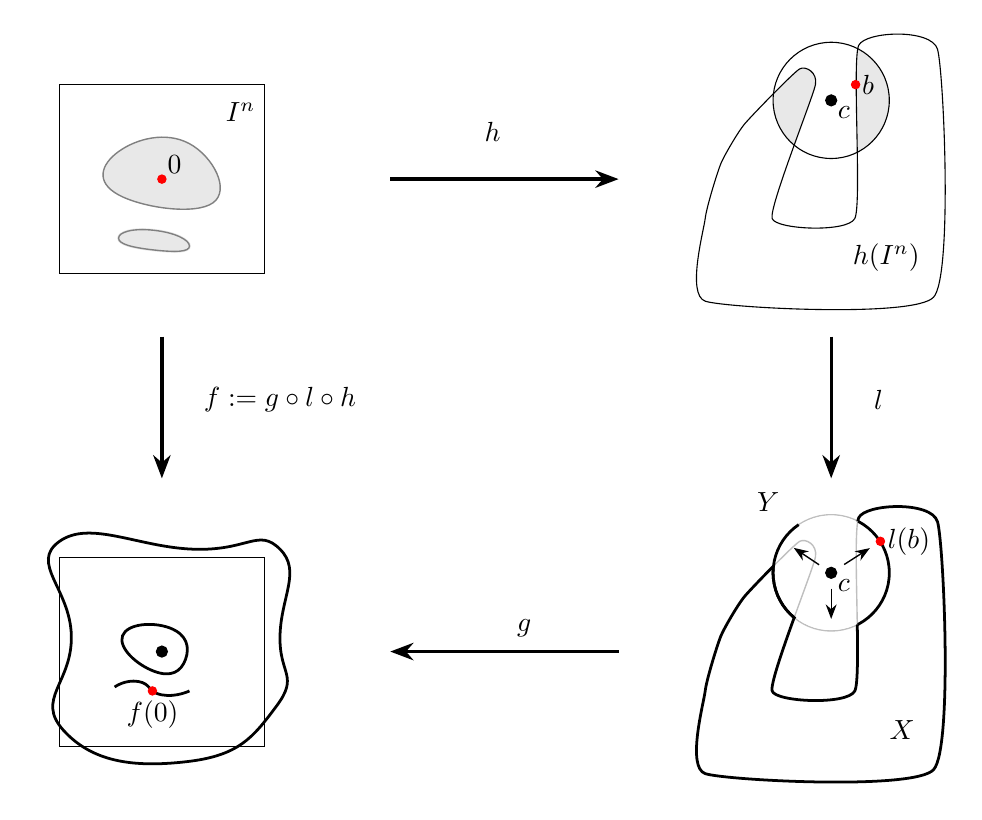
\begin{tikzpicture}
% ###############          prva slika          ###############
		\filldraw[color=gray!18] plot [smooth cycle, tension = 0.9] coordinates {(-5.15, 3.35) (-5.15, 2.8) (-3.95, 2.7) (-4.25, 3.45)};
		\draw[gray, line width=0.5pt] plot [smooth cycle, tension = 0.9] coordinates {(-5.15, 3.35) (-5.15, 2.8) (-3.95, 2.7) (-4.25, 3.45)};
		\filldraw[color=gray!18, line width=1pt] plot [smooth cycle, tension = 1.1] coordinates {(-4.25, 2.15) (-4.7, 2.35) (-5.15, 2.25) (-4.7, 2.1)};
		\draw[gray, line width=0.5pt] plot [smooth cycle, tension = 1.1] coordinates {(-4.25, 2.15) (-4.7, 2.35) (-5.15, 2.25) (-4.7, 2.1)};
		\draw (-5.9, 1.8) rectangle (-3.3, 4.2);
		\filldraw[red] (-4.6, 3) circle (1.5pt) node[black, above right=-0.5mm] {$0$};
		\draw (-4.2, 3.1) ;	
		 \draw (-3.6, 3.85) node {$I^n$};
		
% ###############          druga slika          ###############
		\begin{scope}
			\clip plot [smooth cycle, tension = 0.3] coordinates {(2.3, 1.45) (5.2, 1.5) (5.25, 4.65) (4.25, 4.7) (4.2, 2.5) (3.15, 2.5) (3.7, 4.2) (3.5, 4.4) (2.8,3.7)  (2.5, 3.2) (2.3, 2.5)};
			\clip (3.9, 4) circle (21pt);
			\fill[color=gray!18] (-2,1.5) rectangle (6,5);
		\end{scope}
		\draw plot [smooth cycle, tension = 0.3] coordinates {(2.3, 1.45) (5.2, 1.5) (5.25, 4.65) (4.25, 4.7) (4.2, 2.5) (3.15, 2.5) (3.7, 4.2) (3.5, 4.4) (2.8,3.7)  (2.5, 3.2) (2.3, 2.5)};
		\filldraw[black] (3.9, 4) circle (2pt) node[black, below right=-0.4mm]{$c$};
		\filldraw[red] (4.21, 4.2) circle (1.5pt) node[black, right=-0.4mm] {$b$};
		\draw[black] (3.9, 4) circle (21pt);
		\draw (4.6, 2) node {$h(I^n)$};
	
% ###############          tretja slika          ###############
		\draw[lightgray, line width=0.5pt] (3.9, -2) circle (21pt);
		\draw[black, line width=1pt] plot [smooth cycle, tension = 0.3] coordinates {(2.3, -4.55) (5.2, -4.5) (5.25, -1.35) (4.25, -1.3) (4.2, -3.5) (3.15, -3.5) (3.7, -1.8) (3.5, -1.6) (2.8, -2.3)  (2.5, -2.8) (2.3, -3.5)};
		\filldraw[white] (3.9, -2) circle (20.5pt);
		\begin{scope}
			\clip (3.9, -2) circle (21pt);
			\draw[lightgray, line width=0.5pt] plot [smooth cycle, tension = 0.3] coordinates {(2.3, -4.55) (5.2, -4.5) (5.25, -1.35) (4.25, -1.3) (4.2, -3.5) (3.15, -3.5) (3.7, -1.8) (3.5, -1.6) (2.8, -2.3)  (2.5, -2.8) (2.3, -3.5)};
		\end{scope}
		\begin{scope}
			\clip (3.9, -2) -- (3.4, -1.26) -- (2.5, -1) -- (3.35, -2.7) -- cycle;
			\draw[black, line width=1pt] (3.9, -2) circle (21pt);
		\end{scope}
		\begin{scope}
			\clip plot [smooth cycle, tension = 0.3] coordinates {(2.3, -4.55) (5.2, -4.5) (5.25, -1.35) (4.25, -1.3) (4.2, -3.5) (3.15, -3.5) (3.7, -1.8) (3.5, -1.6) (2.8, -2.3)  (2.5, -2.8) (2.3, -3.5)};
			\draw[black, line width=1pt] (3.9, -2) circle (21pt);
		\end{scope}
		\filldraw[black] (3.9, -2) circle (2pt) node[black, below right=-0.4mm]{$c$};
		\draw[black, line width=0.5pt, -Stealth] ($($(3.9, -2)!.5!(4.525, -1.6)$)!5pt!(3.9, -2)$) --  ($($(3.9, -2)!.5!(4.525, -1.6)$)!6pt!(4.525, -1.6)$);
		\draw[black, line width=0.5pt, -Stealth] ($($(3.9, -2)!.5!((3.9, -2.75)$)!5pt!(3.9, -2)$) --  ($($(3.9, -2)!.5!((3.9, -2.75)$)!6pt!((3.9, -2.75)$);
		\draw[black, line width=0.5pt, -Stealth] ($($(3.9, -2)!.5!(3.3, -1.6)$)!5pt!(3.9, -2)$) --  ($($(3.9, -2)!.5!(3.3, -1.6)$)!6pt!(3.3, -1.6)$);
		\filldraw[red] (4.525, -1.6) circle (1.5pt) node[black, right=-0.3mm] {$l(b)$};
		\draw (3.1, -1.1) node {$Y$};
		\draw (4.8, -4) node {$X$}; 
		
	% ###############          četrta slika          ###############
		\draw (-5.9, -4.2) rectangle (-3.3, -1.8);
		\draw[black, line width=1pt] plot [smooth cycle, tension = 1] coordinates {(-4.5, -2.7) (-4.3, -3.1) (-4.7, -3.25) (-5.1, -2.8)};
		\draw[black, line width=1pt] plot [smooth, tension = 1] coordinates {(-5.2, -3.45) (-4.9, -3.38) (-4.6, -3.55) (-4.25, -3.5)};
		\filldraw[red] (-4.72, -3.5) circle (1.5pt) node[black, below] {$f(0)$};
		\filldraw[black] (-4.6, -3) circle (2pt);
		\draw[black, line width=1pt] plot [smooth cycle, tension = 0.9] coordinates { (-3.1, -1.7) (-4.2, -1.7) (-5.9, -1.6) (-5.75, -2.8) (-5.85, -4) (-4.3, -4.4) (-3.15, -3.7) (-3.1, -2.8)};
	
	% ###############          puščice          ###############
		\draw [black, line width=1.2pt, -Stealth] (-1.7,3) -- (1.2,3);
		\draw (-0.4, 3.6) node {$h$};
		\draw [black,  line width=1.2pt, -Stealth] (1.2, -3) -- (-1.7, -3);
		\draw (0, -2.7) node {$g$};
		\draw [black,  line width=1.2pt, -Stealth] (-4.6, 1) -- (-4.6, -0.8);
		\draw (-3.1, 0.2) node {$f  := g \circ l \circ h$};
		\draw [black,  line width=1.2pt, -Stealth] (3.9, 1) -- (3.9, -0.8);
		\draw (4.5, 0.2) node {$l$};  
	\end{tikzpicture}
	\caption{Skica dokaza izreka \ref{main_theorem}.}
\end{figure}

Označimo $X := h(\I^n) \setminus B(c, \delta)$ in $Y := \partial B(c, \delta)$. Definiramo zvezno preslikavo $l : h(\I^n) \cup Y \to X \cup Y$ s predpisom:
\[  l(x) = \left\{
\begin{array}{ll}
	c + \frac{x - c}{\| x - c \|} \cdot \delta &, x \in h(\I^n) \cup B(c, \delta) \\
	x &, x \in X. \\
\end{array} 
\right. \]
S pomočjo leme \ref{lem:razsiritev-nic} lahko preslikavo $h|_X : X \to \R^n \setminus \{ 0 \}$ do zvezne preslikave $g : X \cup Y \to \R^n \setminus \{ 0 \}$, za katero za vsak $x \in X$ velja $\| g(x) - h^{-1}(x) \| < a$.
Sedaj lahko definiramo preslikavo $f = (f_1, f_2, \dots, f_n) : \I^n \to \R \setminus \{ 0 \}$ kot kompozitum $f := g \circ l \circ h$. Ker ta funkcija slika iz $\I^n$ in ne zavzame ničle, je za protislovje dovolj, če se prepričamo, da funkcija ustreza pogojem izreka \ref{izr:PM}. Vzemimo $t \in \I_i^-$. Velja $l(h(t)) = h(t)$, saj je $h(t) \in X$. Poglejmo normo $\| f(t) - t \| = \| g(l(h(t))) - h{-1}(h(t)) \| = \| g(h(t) - h{-1}(h(t)) \| < a$. Ker je $t_i = - a$ je $| f_i (t) - t_i | = | f_i (t) - ( - a) | \leq | f (t) - t | < a$ torej je $f_i(t) < 0$. Enako lahko sklepamo tudi v primeru, ko je $t_i \in \I_i^+$. Ugotovili smo, da je  $f_i(\I_i^-) < 0$ in $f_i(\I_i^+) > 0$, zato bi po predpostavkah izreka \ref{izr:PM} moral obstajati $x \in \I^n$, ki se z $f$ slika v $0$. To je protislovje, torej je $b \in \Int (h(\I^n)$ in je $h(U)$ odprta podmnožica v $\R^n$.
\end{dokaz}


\begin{izrek}[Izrek o invarianci dimenzije]\label{izr:dim_izr}
Naj bosta $m$ in $n$ naravni števili, potem sta Evklidska prostora $\R^m$ in $\R^n$ homeomorfna, če in samo če je $m = n$.
\end{izrek}

\begin{dokaz}
Denimo, da sta za neki dve naravni števili $m$ in $n$ Evklidska prostora $\R^m$ in $\R^n$ homeomorfna. Torej obstaja zvezna bijektivna preslikava $f : \R^n \to \R^m$ z zveznim inverzom $f^{-1} : \R^m \to \R^n$. Dolazovali bomo s protislovjem. Predpostavimo, da je $m \neq n$, brez izgube splošnosti lahko predpostavimo , da je $m < n$. Označimo z $i$ vložitev, torej preslikavo iz prostora $\R^m$ v $\R^n$, ki je definirana s predpisom $i(x_1, \dots, x_m) = (x_1, \dots, x_m, 0, \dots, 0)$. Tedaj je preslikava $h : \R^n \to \R^n$ definirana kot kompozitum $h := i \circ f$ zvezna injektivna preslikava, zato je po izreku \ref{izr:main-theorem} odprta. Toda slika prostora $\R^n$, ki je odprta podmnožica same sebe, je množica $\left \{ (x_1, x_2, \dots, x_m, 0, \dots, 0) \in \R^n ; \text{ kjer so } x_i \in \R \text{ za vsak } i \in \{1, \dots, m \}  \right \}$, ki pa je zaprta podmnožica prostora $\R^n$. Torej mora biti res $m = n$.
\end{dokaz}

\section*{Slovar strokovnih izrazov}

\geslo{}{}
\geslo{}{}

% seznam uporabljene literature
\begin{thebibliography}{99}

%\bibitem{}

\bibitem{referenca-spletni-vir}
I.~Priimek, \emph{Naslov spletnega vira}, v: ime morebitne zbirke/zbornika, ki vsebuje vir, verzija številka/datum, [ogled datum], dostopno na \url{spletni.naslov}.

\bibitem{glob-splet}
J.~Globevnik in M.~Brojan, \emph{Analiza 1}, verzija 15.~9.~2010, [ogled 12.~5.~2011], dostopno na \url{http://www.fmf.uni-lj.si/~globevnik/skripta.pdf}.

\bibitem{wiki}
\emph{Matrix (mathematics)}, v: Wikipedia, The Free Encyclopedia, [ogled 12.~5.~2011], dostopno na \url{http://en.wikipedia.org/wiki/Matrix_(mathematics)}.

\end{thebibliography}

\end{document}

